\documentclass{article}
\usepackage[final]{colm2026_conference}

\usepackage{amsmath,amssymb,amsthm}
\usepackage{booktabs}
\usepackage{graphicx}
\usepackage{hyperref}
\usepackage{url}
\usepackage{microtype}
\usepackage{xcolor}
\usepackage{lineno}
\usepackage{enumitem}
\usepackage{multirow}
\usepackage{pgfplots}
\pgfplotsset{compat=1.18}

\newtheorem{proposition}{Proposition}
\newcommand{\R}{\mathbb{R}}

\title{\textbf{Where Does Online Low-Rank KV-Cache Compression Help?\\
A Fair Evaluation at 7B and 14B Scale}}

\author{
  David Aror \\
  Independent Research \\
  \texttt{tejirid.aror@gmail.com}
}

\date{}

\begin{document}

\ifcolmsubmission
\linenumbers
\fi

\maketitle

\begin{abstract}
Online low-rank methods compress the key-value (KV) cache by projecting keys
and values onto a small basis maintained while tokens stream in. We evaluate
one such design, TKV (a basis fit during a warmup window and then frozen,
giving $\mathcal{O}(R d)$ per-token cost), against a corrected OjaKV baseline
and the StreamingLLM eviction baseline at \emph{matched KV memory}, on
Mistral-7B and Qwen2.5-14B. Four findings emerge. (1) A frozen basis must be
fit to keys \emph{before} rotary position embedding: compressing post-RoPE
keys roughly doubles the perplexity cost on both models. (2) Low-rank quality
comparisons are fragile to baseline bugs: a stale-coordinate error in a
common Oja's-rule implementation inflates its error beyond that of storing
nothing, while a corrected OjaKV matches TKV within 0.5\%. (3) On
language-modeling perplexity (WikiText-2, PG-19, and a WikiText$\to$code
distribution shift), eviction beats low-rank compression at every memory
budget tested on both models, e.g.\ $+1.0\%$ vs.\ $+5.3$--$5.6\%$ at 0.59$\times$
memory. (4) Low-rank compression can win where eviction cannot: it keeps a
compressed copy of every token, and on Mistral-7B it retrieves needles that
StreamingLLM has evicted (87\% vs.\ 60\% top-1 at 4K tokens) --- but only at high
rank, not on Qwen2.5-14B, and not when memory is traded away from the exact
window. TKV's frozen basis also cuts per-layer GPU decode latency relative to the full
cache at 32K--128K tokens (5.8--7.9$\times$ at rank 32, 2.1--2.2$\times$ at rank 64)
and is 1.5--3.7$\times$ faster than OjaKV's per-token updates at those lengths.
\end{abstract}

%% ============================================================
\section{Introduction}
\label{sec:intro}

The KV cache grows linearly with context and dominates inference memory at
long context. Two families of online methods reduce it without offline
calibration. \emph{Eviction} keeps a subset of tokens exactly, e.g.\ attention
sinks plus a recent window (StreamingLLM, \citealp{streamingllm2023}) or
attention-guided selection \citep{h2o2023,snapkv2024}. \emph{Low-rank
compression} keeps every token but projects keys and values onto a rank-$R$
basis maintained online, as in OjaKV \citep{ojakov2025}, which tracks the basis
with Oja's rule \citep{oja1982}.

This paper studies a simple low-rank design, TKV, which fits the basis during
a bounded warmup window and then freezes it, so each later token costs one
$\mathcal{O}(Rd)$ projection. Rather than report TKV's best case, we ask when
online low-rank compression is worth its cost compared with the obvious
alternatives, under a protocol designed to make the comparison fair: the same
exact sink tokens and recent window for every compressed method, the same
scored tokens, and memory budgets matched byte-for-byte against eviction.

\textbf{Contributions.}
\begin{itemize}[leftmargin=*,itemsep=1pt]
  \item \textbf{Pre-RoPE bases.} A basis frozen on post-RoPE keys cannot span
        keys at later positions; fitting it pre-RoPE and re-applying the
        rotation halves the perplexity cost at 7B and 14B scale
        (Section~\ref{sec:rope}).
  \item \textbf{A corrected OjaKV baseline.} We identify a stale-coordinate bug
        that makes Oja's-rule caches look far worse than they are, and show a
        corrected, equally-initialized OjaKV matches TKV in quality
        (Section~\ref{sec:oja}).
  \item \textbf{Eviction wins on perplexity.} At matched memory StreamingLLM
        beats both low-rank methods on WikiText-2, PG-19, and a
        distribution-shift benchmark, for both models (Section~\ref{sec:ppl}).
  \item \textbf{Low-rank wins some retrieval.} Compressed-but-kept tokens can be
        retrieved after eviction has discarded them, but the effect needs high
        rank and is model-dependent (Section~\ref{sec:retrieval}).
  \item \textbf{GPU decode cost.} A frozen basis makes the per-layer decode step
        5.8--7.9$\times$ (rank 32) and 2.1--2.2$\times$ (rank 64) faster than the
        full cache at 32K--128K tokens (Section~\ref{sec:latency}).
\end{itemize}

%% ============================================================
\section{Methods and Protocol}
\label{sec:method}

\paragraph{Cache layout (shared by all compressed methods).}
For each layer and KV head, query $i$ attends to the first $S$ tokens
(attention sinks) and to a sliding window of the $W$ most recent tokens
\emph{exactly}; every other earlier token is either compressed (low-rank
methods) or evicted (StreamingLLM). We use $S{=}64$ and, for the low-rank
methods, $W{=}256$.

\paragraph{TKV (frozen basis).}
TKV fits rank-$R$ bases $B_K, B_V \in \R^{R\times d}$ to the first
$T_0{=}512$ tokens and freezes them; a later token is stored as its
coefficients $B_K\mathbf{k}, B_V\mathbf{v}$ ($\mathcal{O}(Rd)$), and attention
reads the compressed cache at $\mathcal{O}(R(T{+}d))$ cost. The warmup basis
can be built online from a Halko randomized range finder \citep{halko2011}
followed by Brand's rank-1 SVD updates \citep{brand2006}; in all experiments we
use the exact truncated SVD of the warmup window, which minimizes warmup
reconstruction error and so represents the best case for a streaming warmup
(Appendix~\ref{app:brand}).

\paragraph{Pre-RoPE compression.}
Modern LLMs apply rotary embeddings \citep{rope2021} to keys before attention.
We fit $B_K$ on \emph{pre}-RoPE keys, store pre-RoPE coefficients, and apply
RoPE to the reconstructed key at its own position, as in Palu
\citep{palu2024} and ShadowKV \citep{shadowkv2024}. Values have no positional
rotation. Section~\ref{sec:rope} compares both variants.

\paragraph{OjaKV (corrected).}
Our OjaKV starts from the \emph{same} warmup SVD basis as TKV, then updates the
basis with a normalized Oja step,
$B \leftarrow \mathrm{QR}\bigl(B + \eta_t (B\mathbf{x})\mathbf{x}^\top\bigr)$ with
$\eta_t = 1/\bigl((t{+}1)\lVert\mathbf{x}\rVert^2\bigr)$, every 16 tokens, and
rotates stored coefficients into the new basis so that coefficients and basis
always share a coordinate frame. Each query attends through the basis
available at its own time step (strictly causal).

\paragraph{StreamingLLM at matched memory.}
Per head and layer, a rank-$R$ compressed cache over $T$ tokens stores
$TR + Rd$ coefficient and basis entries per tensor on top of the
$(S{+}W)d$ exact entries. We give StreamingLLM the same bytes as extra window
tokens: $W' = W + TR/d + R$. The reported memory ratio is
$\bigl((TR + Rd) + (S{+}W)d\bigr)/(Td)$, averaged over layers. It charges
coefficients for every token, so it slightly favors eviction; at $T{=}4096$,
$d{=}128$, ranks 16/32/64 give 0.21/0.34/0.59$\times$ memory.

\paragraph{Models and data.}
Mistral-7B-v0.1 \citep{mistral2023} (32 layers, 8 KV heads, $d{=}128$) and
Qwen2.5-14B \citep{qwen25} (48 layers, 8 KV heads, $d{=}128$), in bfloat16.
Perplexity uses the HuggingFace strided protocol with context 4096 and stride
1024 on WikiText-2 test \citep{merity2017} (the full split joined with blank
lines) and on PG-19 test books \citep{rae2020}, 30 windows each (33.8K scored
tokens). The \emph{shift} benchmark builds each 4096-token window from 512
WikiText-2 tokens (the warmup) followed by 3584 tokens of Python code
(codeparrot), so every post-freeze token comes from a domain the basis never
saw (30 windows, 107.5K post-freeze tokens). All methods score the same
tokens; we report perplexity on post-freeze tokens (in-window position
$> T_0$). Compression is simulated in one teacher-forced pass per window with
a custom attention function whose output matches token-by-token streaming
(max abs.\ error $7\times10^{-7}$ in our tests); with $R{=}d$ or
$S{+}W \ge T$ each hook reproduces exact logits.

%% ============================================================
\section{Results}
\label{sec:results}

\subsection{A frozen basis must be fit before RoPE}
\label{sec:rope}

\begin{table}[t]
\centering
\caption{WikiText-2 perplexity (post-freeze tokens), TKV at rank 64
(0.59$\times$ memory), context 4096. Relative increase over exact in parentheses.}
\label{tab:rope}
\small
\begin{tabular}{lccc}
\toprule
& Exact & TKV, post-RoPE basis & TKV, pre-RoPE basis \\
\midrule
Mistral-7B  & 4.595 & 5.124 (+11.5\%) & \textbf{4.853 (+5.6\%)} \\
Qwen2.5-14B & 3.977 & 4.377 (+10.1\%) & \textbf{4.189 (+5.3\%)} \\
\bottomrule
\end{tabular}
\end{table}

RoPE rotates each key by an angle proportional to its position, so a
subspace fitted to positions $0..T_0$ does not span the same keys rotated to
positions far beyond $T_0$. Fitting the basis before RoPE removes this
position dependence and roughly halves the perplexity cost on both models
(Table~\ref{tab:rope}). On a small model the effect is catastrophic: on
TinyLlama-1.1B ($d{=}64$, context 2048) post-RoPE TKV at rank 48 reaches
perplexity 76.3 against 6.86 exact, while pre-RoPE TKV reaches 6.94. All
remaining low-rank results use pre-RoPE bases.

\subsection{A corrected OjaKV matches TKV}
\label{sec:oja}

A natural streaming implementation of Oja's rule stores each token's
coefficients $\mathbf{h}_t = B_t\mathbf{x}_t$ at arrival and reconstructs the
cache as $H B_T$ with the \emph{final} basis. Because the basis rotates after
every update, stored coefficients and basis live in different coordinate
frames; with an unnormalized step ($\eta_t = 1/(t{+}1)$, no division by
$\lVert\mathbf{x}\rVert^2$) and key norms in the tens, the basis nearly snaps
to each new token and the frame mismatch dominates. On real key activations
this produced relative reconstruction errors above 1.0 --- worse than storing
zeros --- and flat across rank, and a perplexity-hook variant that mixed
final-basis queries with stale keys produced perplexities in the hundreds to
thousands. Normalizing the step, rotating coefficients into each new basis, and
initializing from the same warmup SVD as TKV fixes both.

\begin{table}[t]
\centering
\caption{Perplexity (post-freeze) at rank 64, 0.59$\times$ memory. Both
low-rank methods share warmup, sink, and window; StreamingLLM gets the same
bytes as exact window tokens.}
\label{tab:oja}
\small
\begin{tabular}{llcccc}
\toprule
Model & Data & Exact & TKV & OjaKV (corrected) & StreamingLLM \\
\midrule
\multirow{2}{*}{Mistral-7B}  & WikiText-2 & 4.595 & 4.853 (+5.6\%) & 4.835 (+5.2\%) & \textbf{4.640 (+1.0\%)} \\
                             & Shift      & 2.314 & 2.421 (+4.6\%) & 2.412 (+4.2\%) & \textbf{2.318 (+0.2\%)} \\
\midrule
\multirow{2}{*}{Qwen2.5-14B} & WikiText-2 & 3.977 & 4.189 (+5.3\%) & 4.180 (+5.1\%) & \textbf{4.018 (+1.0\%)} \\
                             & Shift      & 2.311 & 2.438 (+5.5\%) & 2.425 (+4.9\%) & \textbf{2.315 (+0.2\%)} \\
\bottomrule
\end{tabular}
\end{table}

With these fixes OjaKV is within 0.5\% of TKV everywhere, and slightly better
(Table~\ref{tab:oja}), including on the shift benchmark where its adaptivity
should help most. TKV's advantage over a correct OjaKV is cost, not quality:
it performs no basis updates after warmup (Section~\ref{sec:latency}).

\subsection{On perplexity, eviction beats low-rank compression}
\label{sec:ppl}

\begin{figure}[t]
\centering
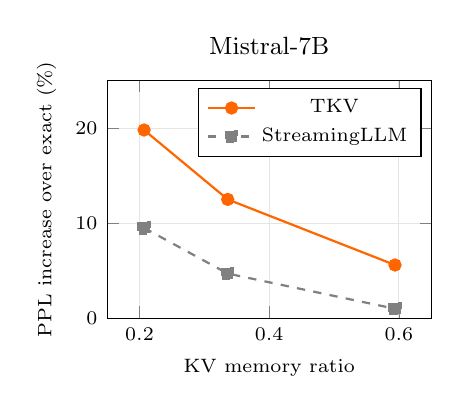
\begin{tikzpicture}
\begin{axis}[
  width=0.47\linewidth, height=4.6cm, title={Mistral-7B}, title style={font=\small},
  xlabel={KV memory ratio}, ylabel={PPL increase over exact (\%)},
  xmin=0.15, xmax=0.65, ymin=0, ymax=25, grid=major, grid style={gray!20},
  tick label style={font=\scriptsize}, label style={font=\scriptsize},
  legend style={font=\scriptsize, at={(0.97,0.97)}, anchor=north east}]
  \addplot[color=orange!80!red, mark=*, thick] coordinates {(0.207,19.8)(0.336,12.5)(0.594,5.6)};
  \addlegendentry{TKV}
  \addplot[color=gray, mark=square*, thick, dashed] coordinates {(0.207,9.5)(0.336,4.7)(0.594,1.0)};
  \addlegendentry{StreamingLLM}
\end{axis}
\end{tikzpicture}\hfill
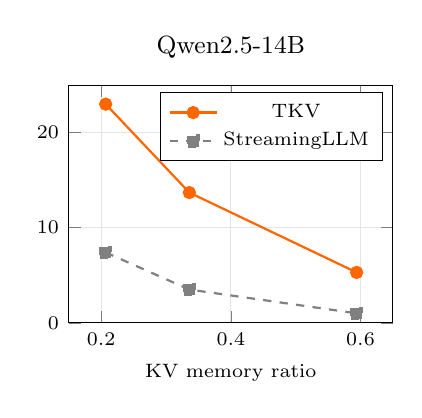
\begin{tikzpicture}
\begin{axis}[
  width=0.47\linewidth, height=4.6cm, title={Qwen2.5-14B}, title style={font=\small},
  xlabel={KV memory ratio},
  xmin=0.15, xmax=0.65, ymin=0, ymax=25, grid=major, grid style={gray!20},
  tick label style={font=\scriptsize}, label style={font=\scriptsize},
  legend style={font=\scriptsize, at={(0.97,0.97)}, anchor=north east}]
  \addplot[color=orange!80!red, mark=*, thick] coordinates {(0.207,23.0)(0.336,13.7)(0.594,5.3)};
  \addlegendentry{TKV}
  \addplot[color=gray, mark=square*, thick, dashed] coordinates {(0.207,7.4)(0.336,3.5)(0.594,1.0)};
  \addlegendentry{StreamingLLM}
\end{axis}
\end{tikzpicture}
\caption{WikiText-2 perplexity increase vs.\ KV memory (ranks 16/32/64 and
matched StreamingLLM windows), context 4096.}
\label{fig:ppl}
\end{figure}

StreamingLLM beats TKV at every memory budget on both models
(Figure~\ref{fig:ppl}), and the gap widens as memory shrinks: at 0.21$\times$
memory TKV costs $+19.8\%$ / $+23.0\%$ perplexity (Mistral / Qwen) against
$+9.5\%$ / $+7.4\%$ for eviction. The same ordering holds on PG-19 at rank 64
(Mistral $+2.5\%$ vs.\ $+0.7\%$; Qwen $+2.3\%$ vs.\ $+0.9\%$) and on the shift
benchmark (Table~\ref{tab:oja}), where the frozen basis sees only code after
fitting on prose. Next-token prediction relies mostly on nearby context, which
eviction keeps exactly and low-rank compression perturbs.

\paragraph{Rank schedule.} A PyramidKV-style \citep{pyramidkv2024} per-layer
schedule (ranks 96/64/48/32 by layer quarter, 0.56$\times$ memory) is worse
than uniform rank 64 at similar memory for TKV (Mistral $+8.0\%$ vs.\ $+5.6\%$;
Qwen $+9.1\%$ vs.\ $+5.3\%$), so we use uniform ranks.

\subsection{Retrieval: where keeping every token matters}
\label{sec:retrieval}

\begin{table}[t]
\centering
\caption{Needle-in-a-haystack top-1 accuracy (5 depths $\times$ 3 needles,
WikiText-2 haystack) at matched memory; SLLM = StreamingLLM with the same KV
bytes. Memory at rank 16: 0.29/0.21/0.17$\times$ (2K/4K/8K); rank 64:
0.69/0.59/0.55$\times$.}
\label{tab:niah}
\small
\begin{tabular}{llccccc}
\toprule
Model & Context & Exact & TKV r16 & SLLM r16 & TKV r64 & SLLM r64 \\
\midrule
\multirow{2}{*}{Mistral-7B}  & 2K & 1.00 & 0.20 & 0.20 & \textbf{0.80} & 0.60 \\
                             & 4K & 1.00 & 0.00 & 0.20 & \textbf{0.87} & 0.60 \\
\midrule
\multirow{2}{*}{Qwen2.5-14B} & 4K & 1.00 & 0.00 & 0.20 & 0.20 & \textbf{0.60} \\
                             & 8K & 1.00 & 0.00 & 0.20 & 0.27 & \textbf{0.60} \\
\bottomrule
\end{tabular}
\end{table}

Perplexity cannot show the one thing eviction gives up: tokens outside the
window are gone. We insert a one-sentence needle (``The special code word is
\emph{blue}.'') into WikiText-2 text at depths 0.1--0.9 and ask for it at the
end \citep{niah2023}. StreamingLLM retrieves the needle only when it lies in its
window (depths $\ge 0.5$ at rank 64) and never at depths 0.1--0.3. On
Mistral-7B, rank-64 TKV also answers many evicted-depth needles, raising top-1
accuracy from 0.60 to 0.87 at 4K tokens (OjaKV: 0.93). This advantage does not
transfer: on Qwen2.5-14B rank-64 TKV mostly fails outside its window (0.20 and
0.27), and at rank 16 no compressed method retrieves anything outside the
window on either model (Table~\ref{tab:niah}). Needles at depth 0.1 of a 4K
context fall inside the 512-token warmup, where the basis was fit on the
needle itself; these are the easiest compressed cases.

\paragraph{Spending memory on rank or on window?}
The cache layout lets a fixed budget be split between a rank-$R$ compressed
middle and an exact window; each unit of rank costs $T/d + 1$ window tokens.
At the rank-64 budget (0.59$\times$, 4K) we swept $R\in\{0,16,32,48,64\}$
with $W = 256 + (64{-}R)(T/d{+}1)$ (Table~\ref{tab:hybrid}). Perplexity
worsens monotonically as memory moves from window to rank on both models.
Retrieval does not recover until $R=64$ on Mistral; at $R\le 32$ the
compressed middle retrieves almost nothing and the shorter window loses needles
the pure-eviction cache kept. A low-rank cache therefore pays off for
retrieval only when it can afford high rank.

\begin{table}[t]
\centering
\caption{Fixed memory (0.59$\times$, context 4096): rank of the compressed
middle vs.\ exact window. WikiText-2 perplexity (post-freeze) / needle top-1
accuracy.}
\label{tab:hybrid}
\small
\begin{tabular}{rrcccc}
\toprule
$R$ & $W$ & \multicolumn{2}{c}{Mistral-7B} & \multicolumn{2}{c}{Qwen2.5-14B} \\
\cmidrule(lr){3-4}\cmidrule(lr){5-6}
& & PPL & Needle acc. & PPL & Needle acc. \\
\midrule
0 (StreamingLLM) & 2368 & \textbf{4.640} & 0.60 & \textbf{4.018} & \textbf{0.60} \\
16 & 1840 & 4.682 & 0.40 & 4.046 & 0.33 \\
32 & 1312 & 4.712 & 0.53 & 4.080 & 0.33 \\
48 &  784 & 4.763 & 0.60 & 4.117 & 0.27 \\
64 (TKV+Sink) & 256 & 4.853 & \textbf{0.87} & 4.189 & 0.20 \\
\bottomrule
\end{tabular}
\end{table}

\subsection{Decode cost on GPU}
\label{sec:latency}

\begin{table}[t]
\centering
\caption{Per-token decode cost for one layer (8 KV heads $\times$ 4 query
heads, $d{=}128$, fp16) on an NVIDIA L40S, in ms: cache update plus attention
read. Exact = full cache.}
\label{tab:latency}
\small
\begin{tabular}{rrccc}
\toprule
Tokens & $R$ & Exact & TKV (frozen) & OjaKV \\
\midrule
4,096   & 32 & 0.25 & 0.25 & 0.95 \\
32,768  & 32 & 2.83 & \textbf{0.36} & 1.31 \\
131,072 & 32 & 12.35 & \textbf{2.14} & 3.33 \\
131,072 & 64 & 12.37 & \textbf{5.75} & 8.88 \\
\bottomrule
\end{tabular}
\end{table}

Table~\ref{tab:latency} times one decode step in isolation. Reading the
frozen-basis cache is 7.9$\times$ (32K) and 5.8$\times$ (128K) faster than
reading the full cache at rank 32, and 2.1--2.2$\times$ faster at rank 64; at 4K
there is no gain. It is 1.5--3.7$\times$ faster than OjaKV at 32K--128K (up to
10.5$\times$ at 4K), since it avoids OjaKV's per-token basis update and
$\mathcal{O}(TR^2)$ coefficient rotation. Note that a matched-memory eviction cache reads a comparable number of
entries, so this speedup is relative to the full cache, not to eviction; we
did not measure end-to-end generation throughput.

%% ============================================================
\section{Discussion and Limitations}
\label{sec:discussion}

\textbf{When to use a low-rank cache.} On these models and budgets, eviction
is the better default for language modeling. Low-rank compression earns its
cost only where information outside the recent window must stay accessible
--- and our results show that this requires high rank (here, half the head
dimension) and depends on the model: Mistral-7B's pre-RoPE keys admit
retrievable rank-64 approximations; Qwen2.5-14B's do not. Among low-rank
designs, freezing the basis loses nothing measurable in quality against a
correct adaptive (Oja) basis, even under an abrupt domain shift, while
avoiding its per-token update cost.

\textbf{Limitations.} Contexts are 2K--8K tokens (Mistral-7B-v0.1 uses a
4096-token sliding window), not the 128K regime that motivates KV
compression; the latency microbenchmark extrapolates to 128K but perplexity
and retrieval do not. Perplexity uses 30 windows per setting and retrieval 15
prompts per cell, without confidence intervals. The warmup basis is an exact
SVD, the best case for a streaming warmup. We compare against one eviction
policy and no quantization baseline (e.g.\ KIVI); attention-guided eviction
(H2O, SnapKV) would likely widen eviction's lead on perplexity and could
change the retrieval picture. Compression is simulated in a teacher-forced
pass, so memory is accounted analytically rather than measured.

%% ============================================================
\section{Related Work}
\label{sec:related}

\textbf{Low-rank KV compression.} Offline methods factorize projections or
caches with calibration data (Palu \citealp{palu2024}; LoRC
\citealp{lorc2024}; xKV \citealp{xkv2025}; SVDq \citealp{svdq2025}); ShadowKV
\citep{shadowkv2024} keeps a low-rank pre-RoPE key cache and offloads values.
OjaKV \citep{ojakov2025} is the closest online method, tracking the basis with
Oja's rule and keeping first and recent tokens exact. Our results agree with
the pre-RoPE design choice of Palu and ShadowKV and suggest online low-rank
methods should be compared against eviction at matched memory.
\textbf{Eviction.} StreamingLLM \citep{streamingllm2023}, H2O \citep{h2o2023},
Scissorhands \citep{scissorhands2023}, SnapKV \citep{snapkv2024}, and PyramidKV
\citep{pyramidkv2024} keep subsets of tokens; eviction reduces $T$ while
low-rank compression reduces $d$, and the two compose, as in the cache layout
used here.

%% ============================================================
\section{Conclusion}

Evaluated fairly --- pre-RoPE bases, a corrected adaptive baseline, and
matched-memory eviction --- online low-rank KV compression is not a better
default than keeping the right tokens exactly: StreamingLLM wins on
perplexity on Mistral-7B and Qwen2.5-14B across datasets and budgets. Its
distinctive property is that nothing is discarded, which can preserve
retrieval of evicted content at high rank on some models, and a frozen basis
makes that property cheap to maintain at decode time. We release the
evaluation harness so that future low-rank methods can be measured against
these baselines.

%% ============================================================
\small
\bibliography{colm2026_conference}
\bibliographystyle{colm2026_conference}

\appendix
\section{Streaming warmup and optimality}
\label{app:brand}

Brand's update \citep{brand2006} computes the exact SVD of $[A;\mathbf{x}^\top]$
from the SVD of $A$. A \emph{rank-truncated} streaming variant keeps only the
top $R$ components after each update, i.e.\ it updates the truncation
$A_R$ rather than $A$. This is not, in general, the best rank-$R$
approximation of the full matrix: a direction discarded at step $t$ can become
dominant after later tokens arrive, and the streaming state can no longer
recover it, whereas the batch SVD of all rows would. By the
Eckart--Young--Mirsky theorem \citep{eckart1936,mirsky1960} the exact truncated
SVD of the warmup window is therefore a lower bound on the reconstruction
error of any rank-$R$ streaming warmup, which is why we use it in all
experiments. Because this optimality concerns reconstruction of the warmup
window rather than downstream perplexity, the reported TKV numbers are best
read as a likely-optimistic estimate for a fully streaming implementation.

\section{Additional numbers}
\label{app:numbers}

\textbf{Perplexity at lower memory (WikiText-2, post-freeze).}
Mistral-7B: TKV rank 16/32 = 5.505/5.168 ($+19.8\%/{+}12.5\%$), StreamingLLM
matched = 5.031/4.813 ($+9.5\%/{+}4.7\%$). Qwen2.5-14B: TKV 4.890/4.522
($+23.0\%/{+}13.7\%$), StreamingLLM 4.270/4.115 ($+7.4\%/{+}3.5\%$). Shift, rank
16 (0.21$\times$): TKV $+18.6\%$ / $+18.5\%$, StreamingLLM $+4.3\%$ / $+5.0\%$
(Mistral / Qwen). PG-19, rank 64: exact 5.732 / 6.330, TKV 5.878 / 6.478,
StreamingLLM 5.770 / 6.384.

\textbf{Needle probability by depth (Mistral-7B, 4K, rank 64).}
Mean $P(\text{needle})$ at depths 0.1/0.3/0.5/0.7/0.9: exact
0.69/0.76/0.76/0.75/0.83; TKV 0.60/0.39/0.41/0.28/0.27; OjaKV
0.63/0.40/0.41/0.29/0.27; StreamingLLM 0.00/0.00/0.77/0.77/0.84.

\textbf{Decode latency at rank 64.} 4K: exact 0.25, TKV 0.25, OjaKV 2.61 ms;
32K: 2.84, 1.35, 3.90 ms.

\end{document}
